\section{Réalisation et implémentation}

J'ai choisi de ne pas présenter l'implémentation faite partie par partie, mais de présenter l'implémentation finale car elle contient les éléments correspondant à chacune des parties. 

\subsection{Ajout des PIOs}

Voici ce que l'on peut voir quand on ouvre le projet Qsys qui a été créé : 

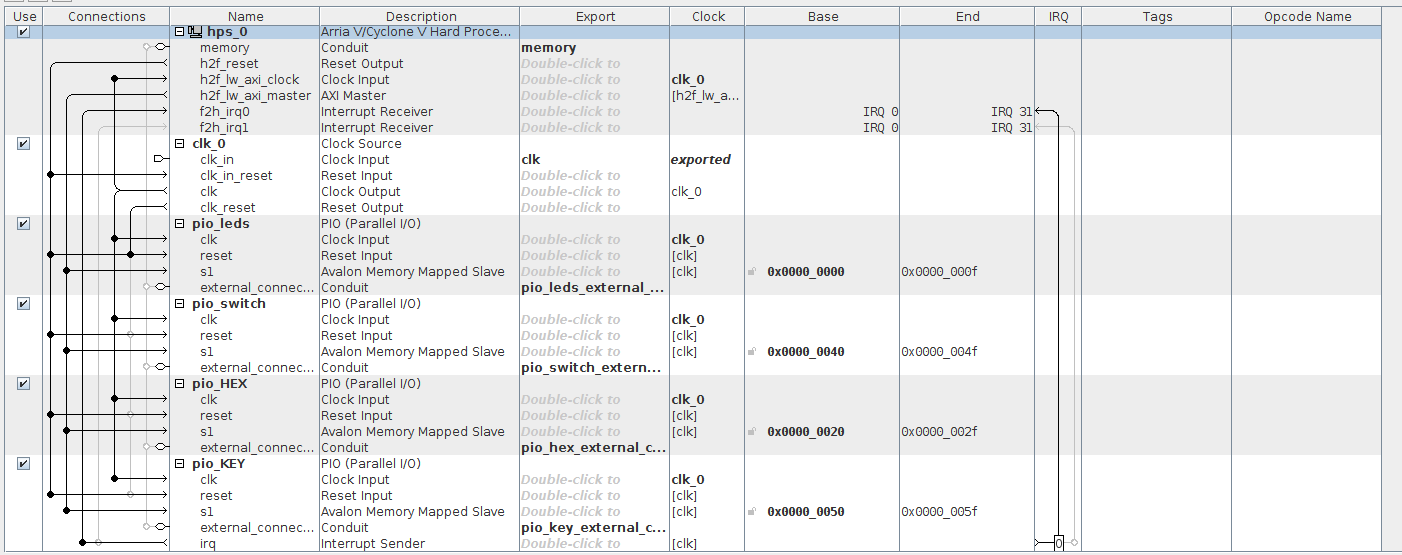
\includegraphics[scale=0.3]{./images/pios.png}
\captionof{figure}{Laboratoire 2 : PIOs}

On peut voir que 4 parallel I/O (pio) ont été ajoutés, un pour chacun des éléments de notre système que l'on souhaitait gérer.\\

La configuration de ces pio est la suivante : \\

\begin{itemize}
	\item pio\_leds : une longueur de 10 (Pour les 10 leds) et set en output
	\item pio\_switch : une longueur de 10 (Pour les 10 switchs) et set en input
	\item pio\_HEX : une longueur de 32 (8 bits par afficheur, avec 2 bits non utilisé, donc 4*8 = 32) et set en output
	\item pio\_KEY: un longueur de 4(Pour les 4 boutons), set en input, avec l'edge capture en rising (Pour récupérer l'appui sur le bouton) et avec les irq actives(irq de type EDGE, afin de se basé sur l'état de l'edge capture pour créer une interruption)\\
\end{itemize}

Le câblage avec les autres éléments consistait à brancher toutes les clocks sur la clock du hps, ainsi que les resets (sur le reset du hps). De plus, pour le cas des KEYs, l'interruption est branchée sur la première "banque" d'interruption de la fpga qui va sur le hps (f2h\_irq0).

La génération du VHDL s'est passé sans problème, et j'ai dû ajouter les pio que j'avais créés au fichier DE1\_SoC\_top.vhd. Pour ce faire, j'ai utilisé qsys et "Show instantiation template" : 

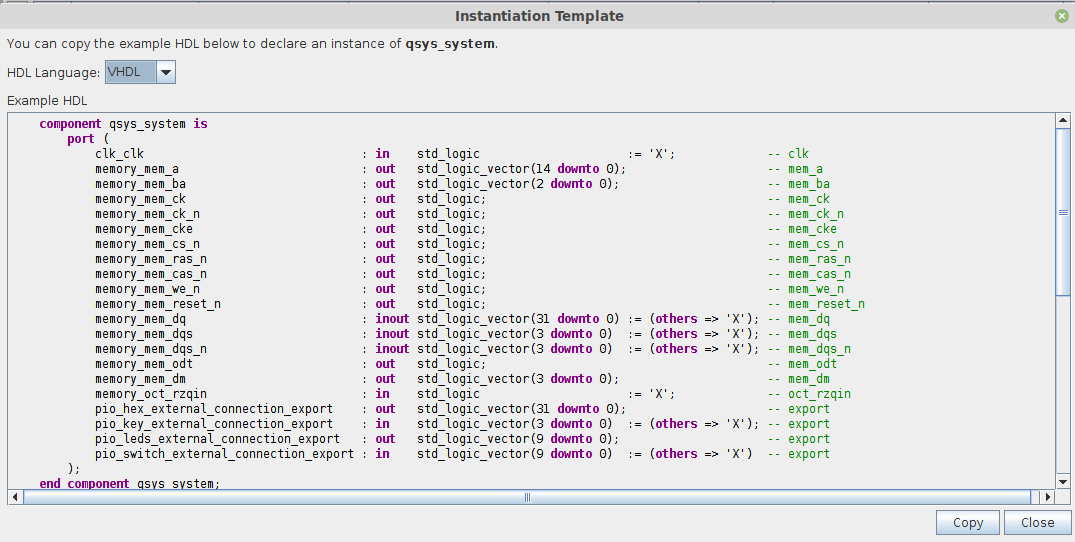
\includegraphics[scale=0.4]{./images/show_instantiation_template.png}
\captionof{figure}{Laboratoire 2 : Instantiation template}

et j'ai ensuite modifié le fichier DE1\_SoC\_top.vhd afin de permettre l'utilisation des pios. J'ai copié les lignes que j'avais trouvées dans l'instanciation template et je les ai mises dans l'import du composant qsys\_system dans le fichier DE1\_Soc\_top. De plus, j'ai dû mapper les entrées et sorties du composant dans le même fichier : 
\begin{lstlisting}[language=VHDL]
System : component qsys_system
port map (
------------------------------------
-- FPGA Side
------------------------------------

-- Global signals

------------------------------------
-- HPS Side
------------------------------------
-- DDR3 SDRAM
clk_clk                               => CLOCK_50_i,
pio_leds_external_connection_export   => LEDR_o,
pio_switch_external_connection_export => SW_I,
pio_hex_external_connection_export    => temp_hex_s,
pio_key_external_connection_export    => KEY_i,
memory_mem_a        => HPS_DDR3_ADDR_o,
memory_mem_ba       => HPS_DDR3_BA_o,
memory_mem_ck       => HPS_DDR3_CK_P_o,
memory_mem_ck_n     => HPS_DDR3_CK_N_o,
memory_mem_cke      => HPS_DDR3_CKE_o,
memory_mem_cs_n     => HPS_DDR3_CS_N_o,
memory_mem_ras_n    => HPS_DDR3_RAS_N_o,
memory_mem_cas_n    => HPS_DDR3_CAS_N_o,
memory_mem_we_n     => HPS_DDR3_WE_N_o,
memory_mem_reset_n  => HPS_DDR3_RESET_N_o,
memory_mem_dq       => HPS_DDR3_DQ_io,
memory_mem_dqs      => HPS_DDR3_DQS_P_io,
memory_mem_dqs_n    => HPS_DDR3_DQS_N_io,
memory_mem_odt      => HPS_DDR3_ODT_o,
memory_mem_dm       => HPS_DDR3_DM_o,
memory_oct_rzqin    => HPS_DDR3_RZQ_i
);

HEX0_o <= temp_hex_s(6 downto 0);
HEX1_o <= temp_hex_s(14 downto 8);
HEX2_o <= temp_hex_s(22 downto 16);
HEX3_o <= temp_hex_s(30 downto 24);

\end{lstlisting}

Comme on peut le voir ci-dessus, j'ai de plus dû créer un signal temporaire permettant de dispatcher la sortie du pio HEX entre les différentes sorties HEX qui étaient présentes dans le fichier.

\subsection{Activation des interruptions dans Qsys}
Dans Qsys, plusieurs configurations devaient être effectuées afin de pouvoir utiliser les interruptions. Voici une liste des démarches effectuées : \\

\begin{itemize}
	\item Il faut activer dans la configuration de hps\_0 , sous "Fpga inteface" -> "interrupts", l'option "Enable FPGA-to-HPS interrupts"
	\item le/les PIO qui doit bénéficier des interruptions doit être linké sur l'un des deux champs "f2h\_irq0/1".
	\item Dans la colonne IRQ aussi, l'interruption du pio doit être linkée sur l'un des deux champs vu plus haut. Dans notre cas, l'interruption porte le numéro 0 et est linkée sur "f2h\_irq0", ce qui implique que le numéro de l'interruption sera le numéro 0 de la fpga( L'image ci-dessous montre le numéro de l'interruption, qui est donc 72)\\
\end{itemize}

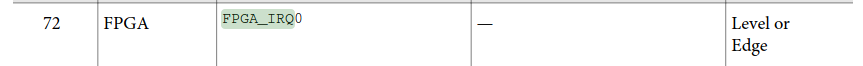
\includegraphics[scale=0.5]{./images/fpga_irq0.png}
\captionof{figure}{Laboratoire 2 : Numéro de l'interruption}

Voici les modifications qui étaient nécessaire dans Qsys afin d'activer les interruptions (En plus de celle déja configurée lors de la création des pios)

\subsection{Programme pour les features sans interruption}
Le fonctionnement du programme pour les parties 1 et 2 du laboratoire a été entièrement commenté directement dans le code. \\
\begin{lstlisting}[language=C]
    while(1)
{
	// Si on appuie sur le Bouton KEY1
	if(!(KEYS & 0x1))
	{
		// On eteind les leds et l'afficheur 7 segements
		LEDS = 0x0;
		HEX3_0 = ~0x0;
		
		// On reporte l'état des switchs sur les leds
		LEDS = SWITCHS;
		
		// On effectue les manipulations demandées pour l'afficheur 7 segements pour KEY1
		HEX3_0 = ~(0x0 | (temp[(LEDS & 0x200) >> 9] << 24) | (temp[(LEDS & 0x100) >> 8] << 16) | (temp[(LEDS & 0xF0) >> 4 ] << 8) | (temp[(LEDS & 0xF)]));
	
	}
	// Si on appuie sur le bouton KEY2
	else if(!(KEYS & 0x2))
	{
		// On eteind les leds et l'afficheur 7 segements
		LEDS = 0x0;
		HEX3_0 = ~0x0;
		
		// On reporte l'état des switchs sur les leds
		LEDS = ~SWITCHS;
		
		// On effectue les manipulations demandées pour l'afficheur 7 segements pour KEY2
		HEX3_0 = ~(0x0 | (temp[(LEDS & 0x200) >> 9] << 24) | (temp[(LEDS & 0x100) >> 8] << 16) | (temp[(LEDS & 0xF0) >> 4 ] << 8) | (temp[(LEDS & 0xF)]));
	}
}
\end{lstlisting}

\subsection{Activation des registres du GIC et de la FPGA dans le code }
Nous allons nous intéresser ici aux valeurs attribuées aux registres dans la partie de code ci-dessous (Les commentaires expliquent le choix des valeurs) : \\

\begin{lstlisting}[language=C]
// Initialize the banked stack pointer register for IRQ mode
set_A9_IRQ_stack();

// On active l'envoi d'interruption au core via l'interface CPU 0
ICCICR = 1;

// On met le niveau nécéssaire pour qu'une interruption soit transmise au cpu au minimum afin que toutes les interruptions passent.
ICCPMR = 0xFFFF;

// On active le distributeur
ICDDCR = 1;

// On calcule la valeur à mettre dans le registre ICDISER (Interrupt Set Enable Registers) et on remplit le registre
// Le calcul pour la valeur peut être trouvé dans le document sous source dans l'entête.
value = 0x1<<(72%32); 
ICDISER |= value;

//On renseigne que notre interruption doit être envoyée à l'interface CPU 0
ICDIPTR = 1;


// On active les interruptions pour les boutons KEY3 et KEY2
KEYS_INTERRUPT_ENABLE = 0xC;

// On active les interruptions sur le processeur
enable_A9_interrupts();
\end{lstlisting}


\subsection{Routine d'interruption}

Voici la routine d'interruption qui a été mise en place pour ce laboratoire :\\
 
\begin{lstlisting}[language=C]
// Define the IRQ exception handler
void __attribute__ ((interrupt)) __cs3_isr_irq(void)
{
	// On lit le registre de l'interface CPU pour savoir quel périphérique a causé l'interruption 
	int interrupt_ID = ICCIAR;
	int hex_val, press;
	
	press = KEYS_INTERRUPT_REGISTER;     // On récupère le bouton qui à causer l'interruption
	KEYS_INTERRUPT_REGISTER = press;     // On nettoie l'interruption dans le registre des interruptions pour les KEYS
	
	// Si l'interruption à été causer par un bouton
	if(interrupt_ID == 72)
	{
		if (press & 0x4)       // KEY2
		{
			// On deplace les leds vers la droite ainsi que les valeurs des afficheurs 7 segments
			LEDS = (LEDS >> 1) | ((LEDS & (0x1 ))<<9);
			hex_val = HEX3_0;
			HEX3_0 = ~0x0;
			HEX3_0 = (0x0 | ((hex_val & (0x7F)) << 24) | ((hex_val & (0x7F << 24)) >> 8) | ((hex_val & (0x7F << 16)) >> 8) | ((hex_val & (0x7F << 8))>>8));
		}
		
		else if (press & 0x8)	// KEY3
		{
			// On deplace les leds vers la gauche ainsi que les valeurs des afficheurs 7 segments
			LEDS = (LEDS << 1) | ((LEDS & (0x1 << 9))>>9);
			hex_val = HEX3_0;
			HEX3_0 = ~0x0;
			HEX3_0 = (0x0 | ((hex_val & (0x7F << 16)) << 8) | ((hex_val & (0x7F << 8)) << 8) | ((hex_val & (0x7F )) << 8) | ((hex_val & (0x7F << 24))>>24));
		}
	
	}
	
	// On nettoie l'interruption dans le registre de interruptions pour le processeur
	ICCEOIR = interrupt_ID;
	return;
}
\end{lstlisting}